% Chapter Template
\part{Adversarial Attacks}

\label{Chapter2} % Change X to a consecutive number; for referencing this chapter 

\section{Adversarial Attacks}

\begin{frame}
  \frametitle{Intriguing Properties of Neural Networks \cite{Szegedy2013}}
\begin{figure}[H]
    \centering
\includegraphics[width=5.5cm]{szegedy/negative1.png}\includegraphics[width=5.5cm]{szegedy/negative2.png}
    \caption{Natural Images are in columns 1 and 4, Adversarial images are in columns 3 and 6, and the difference between them (magnified by a factor of 10) is in columns 2 and 5. All images in columns 3 and 6 are classified by AlexNet as "Ostrich" \cite{Szegedy2013}}
    \label{fig:my_label}
\end{figure}
\end{frame}



%%%%%%%%%%%%%%%%%%%%%%%%%%%%%%%%%%%%%%%%%%%(2)
% 2. define classifier
\begin{frame}
\frametitle{Attacks : L-BFGS}
Let $f : \R^m \to \{1,...,k\}$ be a classifier and assume $f$ has an associated continuous loss function denoted by loss$_f : \R^m \times \{1,...,k\} \to \R^+$ and $l$ a target adversarial . \\
\textbf{ Minimize} $\Norm{r}_2$ subject to:
\begin{enumerate}[1.]
\item $f(x + r) = l$
\item $x + r \in [0,1]^m$
\end{enumerate}

The solution is approximated with L-BFGS as implemented in Pytorch or Keras. This technique yields examples that are close to their original counterparts in the $L^2$ sense.
\end{frame}
\begin{frame}{Attacks : L-BFGS : MNIST}
    \begin{figure}[H]
\label{lbfgsa}
\includegraphics[trim=200 185 100 200, clip, width=6cm]{2019-04-10-adverse/mnist_examples/FC200-200-10-2448-O8-A0-attack_summary.png}\includegraphics[trim=200 185 100 200, clip,width=6cm]{2019-04-10-adverse/mnist_examples/FC200-200-10-2448-O8-A1-attack_summary.png}
\includegraphics[trim=200 185 100 200, clip,width=6cm]{2019-04-10-adverse/mnist_examples/FC200-200-10-2448-O8-A2-attack_summary.png}\includegraphics[trim=200 185 100 200, clip,width=6cm]{2019-04-10-adverse/mnist_examples/FC200-200-10-2448-O8-A3-attack_summary.png}
\includegraphics[trim=200 185 100 200, clip,width=6cm]{2019-04-10-adverse/mnist_examples/FC200-200-10-2448-O8-A4-attack_summary.png}\includegraphics[trim=200 185 100 200, clip,width=6cm]{2019-04-10-adverse/mnist_examples/FC200-200-10-2448-O8-A5-attack_summary.png}
\caption{Original images on the left, Perturbation is in the middle, Adversarial Image (total of Original with Perturbation) is on the right. Column 1 shows an original 8 being perturbed to adversarial classes 0, 2, and 4. Column 2 shows adversarial classes 1, 3, and 5}
\end{figure}
\end{frame}
\begin{frame}{Attacks : Distortion}
    Borrowing a metric from Szegedy et al to compare the magnitude of these distortions, we will define
\begin{definition}{Distortion is the $L^2$ norm of the difference between an original image and a perturbed image, divided by the square root of the number of pixels in the image: }
\[\sqrt{\dfrac{\sum_i \hat (x_i - x_i)^2}{n}}\]
\end{definition}
Distortion is $L^2$ magnitude normalized by the square-root of the number of dimensions so that values can be compared for modeling problems with differing numbers of dimensions. 
\end{frame}

\begin{frame}{Attacks : L-BFGS : MNIST}
    \begin{figure}[H]
\label{lbfgsh}
\includegraphics[trim=200 80 100 100, clip, width=12cm]{2019-04-10-adverse/mnist_examples/FC200-200-10-distortion_hist.png}
\caption{A histogram of the distortion measured for each of 900 adversarial examples generated using L-BFGS against the FC-200-200-10 network on Mnist. Mean distortion is 0.089.}
\end{figure}
\end{frame}
%%%%%%%%%%%%%%%%%%%%%%%%%%%%%%%%%%%%%%%%%%%%%%%%%%%%%%%(3)

\begin{frame}{Attacks : L-BFGS : ImageNet}
 \begin{figure}[H]
\label{lbfgsis}
\includegraphics[trim=200 185 100 200, clip, width=6cm]{2019-04-10-adverse/imnet_examples/vgg16-ILSVRC2012_val_00039098-O722-A965-attack_summary.png}\includegraphics[trim=200 185 100 200, clip, width=6cm]{2019-04-10-adverse/imnet_examples/vgg16-ILSVRC2012_val_00027142-O52-A347-attack_summary.png}
\includegraphics[trim=200 185 100 200, clip, width=6cm]{2019-04-10-adverse/imnet_examples/vgg16-ILSVRC2012_val_00029901-O425-A468-attack_summary.png}\includegraphics[trim=200 185 100 200, clip, width=6cm]{2019-04-10-adverse/imnet_examples/ILSVRC2012_val_00001375-Otensor([42])-A694-attack_summary.png}
% \includegraphics[width=7cm]{2019-04-10-adverse/imnet_examples/vgg16-ILSVRC2012_val_00035978-O803-A353-attack_summary.png}
% \includegraphics[width=7cm]{2019-04-10-adverse/imnet_examples/ILSVRC2012_val_00000886-Otensor([940])-A684-attack_summary.png}
\caption{Original images on the left, Perturbation (magnified by a factor of 100) by is in the middle, Adversarial Image (total of Original with Perturbation) is on the right. Adversarial classes are Burrito, Bison, Taxi, and Paddle Wheel (Top Left, Top Right, Bottom Left, Bottom Right)}
\end{figure}   
\end{frame}

\begin{frame}{Attacks : L-BFGS : ImageNet}
    \begin{figure}[H]
\label{lbfgsi}
\includegraphics[trim=200 80 100 100, clip,width=12cm]{2019-04-10-adverse/imnet_examples/distortion_hist.png}
\caption{A histogram of the distortion measured for each of 112 adversarial examples generated using L-BFGS against the VGG16 network on ImageNet images with mean distortion 0.0107}
\end{figure}
\end{frame}

% 3. discuss solving neural networks, i.e. tuning weights. (gradient and
%    back propagation passes error through the network)
% 4. discus doing this computationally with torch or other
%    multi-threading tools
%%%%%%%%%%%%%%%%%%%%%%%%%%%%%%%%%%%%%%%%%%%%%%%%%%%%%%%%%%%%%%(2)
\begin{frame}
\frametitle{Attacks : FGSM}
A single step attack process using the gradient of the loss function $L$ with respect to an image to find the adversarial perturbation \cite{goodfellow_explaining_2014}. for given $\e$, the modified image $\hat x$ is computed as
\begin{equation}
\hat{x} = x + \epsilon \text{sign} (\nabla L (P_w(x),x))
\end{equation}

This method is simpler and much faster to compute than the L-BFGS technique described above, but produces adversarial examples less reliably and with generally larger distortion.

\end{frame}

\begin{frame}
\frametitle{Attacks : IGSM}
In \cite{kurakin_adversarial_2016}
  an iterative application of FGSM was proposed. After each
  iteration, the image is clipped to a $\e L_\infty$ neighborhood of the original. Let $x'_0 = x$, then after $m$ iterations, the adversarial image obtained is:
\begin{equation}
x_{m+1}' = \text{Clip}_{x,\epsilon} \Bigl\{x_m' + \alpha \times \text{sign}(\nabla \ell (F(x'_m),x'_m))  \Bigr\} 
\label{igsm}
\end{equation}
This method is faster than L-BFGS and more reliable than FGSM but still produces examples with greater distortion than L-BFGS. 
\end{frame}

\begin{frame}{Attacks : IGSM : ImageNet}
    \begin{figure}[H]
  \centering
\includegraphics[trim=200 780 1200 212, clip,width=4cm]{2019-04-10-adverse/ILSVRC2012_val_00002900summary_plot.png}\includegraphics[trim=900 780 500 212, clip,width=4cm]{2019-04-10-adverse/ILSVRC2012_val_00002900summary_plot.png}
%\includegraphics[width=12cm]{2019-04-10-adverse/ILSVRC2012_val_00048234summary_plot.png}
\caption{adversarial example generated against VGG16 (ImageNet) with IGSM. Original Image (Rose Hip) on the left, adversarial image (Baseball) on the right. }
\label{fgsmhip}
\end{figure}
\end{frame}


%\section{Introduction}
%%%%%%%%%%%%%%%%%%%%%%%%%%%%%%%%%%%%%%%%%%%%%%%%%%%%%%%%%%%%%%(2)

% Deep Neural Networks (DNNs) and their variants are core to the success
% of modern machine learning as summarized by ~\citet{prakash2018}. They
% have dominated competitions in image processing, optical character
% recognition, object detection, video classification, natural language
% processing, and many other fields ~\citet{SCHMIDHUBER201585}. Ten years
% ago, along the explosion of applications, an interesting property of
% such networks was observed by ~\citet{szegedy2013}. Their approach was to define a loss function
% relating the output of the ANN for a given initial image to a target adversarial 
% output plus the $L^2$-norm of the input and use backpropagation to
% compute gradients -- not on the weights of the neural network, but on
% just the input layer to the network. The solution to this optimization
% problem, efficiently approximated by a gradient-based optimizer, would
% be a slightly perturbed natural input with a highly perturbed
% output. Their experimental results are striking which we can see in
% Figure.~\ref{fig:szegedy}.  More mysteriously, these examples
% are often transferable -- an attack generated against one
% model may succeed against a totally different model. With the
% incredible expansion of the application of universal function
% approximators in machine-learning, their reliability has come to have
% real-world significance. The ability of an image processing vehicle to
% distinguish speed limit versus stop-signs ~\citep{DBLP:journals/corr/EvtimovEFKLPRS17},
% optimization based models are increasingly relied upon by the defense
% intelligence apparatus ~\citep{hutchins2011intelligence}, search
% engines use ML increasingly to
% determine which sources will receive attention when we ask questions
% and even our personal information security may rely on the robustness
% of machine-learning models against adversarial perturbations. In order
% to wisely use these tools, it is crucial that we carefully understand
% their limitations. It is for this reason that mathematical study and
% formulation of the Adversarial problem is critical. 


% Adversarial examples occur when natural data can be perturbed in small
% ways in order to produce a similar input which receives a
% significantly different model output. ``Small'' in this context may
% refer to small in a particular metric or sometimes is referred to in
% the context of human perception. It is important to note that Adversarial
% examples are not just a peculiarity, but seem to occur for most, if
% not all, DNN  classifiers. For example, ~\citet{inevitable2018} used
% isoperimetric inequalities on high dimensional spheres and hypercubes
% to conclude that there is a reasonably high probability that each
% correctly classified data point has a nearby adversarial
% example. ~\citet{ilyas2019adversarial} argued that optimized models use
% some subtle features for classification which are neither intuitive to
% humans nor robust to perturbation. In particular, that ML models can
% efficiently extract features from training data, but that they do not
% connect these features robustly across scales. The prevalence of these
% features is illustrated by ~\citet{madry2018towards} with the simple experiment of adding vast
% quantities of adversarially perturbed data during training
% . Although this method increases
% adversarial robustness at a cost to prediction accuracy ~\citep{tsipras2018robustness}, it does not
% do so very significantly, and leaves behind vulnerabilities that can
% still be reduced to non-robust features ~\citep{inevitable2018}. 

% %There are now a wide variety of attacks which produce adversarial examples and defenses which try to detect them. \todo{[DG]: not sure this is necessary. [K]: This paragraph is incomplete. Do you think there shouldn't be such a paragraph at all? [DG]: Not sure it is needed. If so, it maybe should probably come right at the beginning before the shafahi/are adversarial examples inevitable.}

% For this work, we will take a geometric approach to analyzing 
% robustness, both in terms of the models' understanding of underlying
% data geometry and by carefully defining the decision boundary of a
% model and studying its properties. In this vein, there have been many
% attempts to identify adversarial examples using properties of the
% decision boundary.  ~\citet{Fawzi2018empirical} found that decision
% boundaries tend to have highly curved regions, and these regions tend
% to favor negative curvature, indicating that regions that define
% classes are highly nonconvex. These were found for a variety of DNNs
% and classification  tasks. 
% %They also suggest exploiting this curvature discrepancy to identify when a data point is a natural image and when it is adversarial. 
% A related idea is that adversarial examples often arise within cones, outside of which images are classified in the original class, as observed by ~\citet{roth19aodds}. Many theoretical models of adversarial examples, for instance the dimple model developed by ~\citet{shamir2021}, have high curvature and/or sharp corners as an essential piece of why adversarial examples can exists very close to natural examples.


% \begin{figure}[H]
%     \centering
% \includegraphics[width=7.3cm]{c1_figures/negative1.png}\includegraphics[width=7.3cm]{c1_figures/negative2.png}
%     \caption{Natural Images are in columns 1 and 4, Adversarial images are in columns 3 and 6, and the difference between them (magnified by a factor of 10) is in columns 2 and 5. All images in columns 3 and 6 are classified by AlexNet as "Ostrich" ~\citep{szegedy2013}.}
%     \label{fig:szegedy}
% \end{figure}

% \section{Common Datasets}

% The first step in all machine-learning and in our endeavor to
% understand adversarial attacks is to understand the data on which
% neural networks are built. We will limit our investigation mostly to
% classic image classification problems, although several of our results
% will hold more generally. The Dataset used above in
% Figure.~\ref{fig:szegedy} is known as ImageNet -- a large set of
% labeled images varying in size originally compiled for the ImageNet
% Large Scale Visual Recognition Challenge (ILSVRC ~\citet{ILSVRC15}). This
% dataset and its many subsets has become a standard for image
% classification and feature identification experiments. In the
% experiments that follow, ImageNet will be featured alongside the
% Modified National Institute of Standards and Technology dataset (MNIST ~\citet{MNIST}) which is a database of hand written digits often used to develop image processing and character recognition systems. This dataset is much lower resolution than ImageNet and is therefore experiments run much more quickly on it and require less complex input/output.  

% \section{Common Attack Techniques}
% % TODO : Add massive carlini toolkit reference
% Adversarial attacks are generally produced by introducing an objective
% function which balances the adversarial objective, e.g. \emph{cross-entropy
% loss} defined by ~\citet{good1963maximum} of the source image as a positive
% value to be minimized or with a specific target combined with a
% regularization term in image space (e.g. the $L^2$ norm) which
% penalizes the generated adversary for being too far from its starting
% point. This loss function is combined with an optimization algorithm
% in order to produce an attack. 


% \subsection{L-BFGS minimizing distortion}\label{lbfgs}

% The original attack used by ~\citet{szegedy2013} took advantage of the
% tools they had on  hand for training neural networks to set up a
% box-constrained optimization problem whose approximated solution
% generates these targeted mis-classifications. We will write this
% precisely according to their formulation: \\

% Let $f : \R^m \to \{1,...,k\}$ be a classifier and assume $f$ has an associated continuous loss function denoted by loss$_f : \R^m \times \{1,...,k\} \to \R^+$ and $l$ a target adversarial . \\
% \textbf{ Minimize} $\Norm{r}_2$ subject to:
% \begin{enumerate}[1.]
% \item $f(x + r) = l$
% \item $x + r \in [0,1]^m$
% \end{enumerate}

% The solution is approximated with L-BFGS (see Appendix \ref{appa}) as
% implemented in Pytorch or Keras. This technique yields examples that
% are close to their original counterparts in the $L^2$ sense, but are
% predicted to be another class by the model with high confidence .  \\

% %Find the minimum $c > 0$ for which the minimizer $r$ of the following satisfies $f(x+r) = l$\\

% %minimize $c|r| + $loss$_f(x+r,l)$ subject to $x + r \in [0,1]^m$.

% \paragraph{L-BFGS: Mnist}
% The following examples are prepared by implementing the above technique via pytorch on images from the Mnist dataset with FC200-200-10, a neural network with 2 hidden layers with 200 nodes each:
% \begin{figure}[H]
% \label{lbfgsa}
% \includegraphics[trim=200 185 100 200, clip, width=7cm]{c1_figures/FC200-200-10-2448-O8-A0-attack_summary.png}\includegraphics[trim=200 185 100 200, clip,width=7cm]{c1_figures/FC200-200-10-2448-O8-A1-attack_summary.png}
% \includegraphics[trim=200 185 100 200, clip,width=7cm]{c1_figures/FC200-200-10-2448-O8-A2-attack_summary.png}\includegraphics[trim=200 185 100 200, clip,width=7cm]{c1_figures/FC200-200-10-2448-O8-A3-attack_summary.png}
% \includegraphics[trim=200 185 100 200, clip,width=7cm]{c1_figures/FC200-200-10-2448-O8-A4-attack_summary.png}\includegraphics[trim=200 185 100 200, clip,width=7cm]{c1_figures/FC200-200-10-2448-O8-A5-attack_summary.png}
% \caption{Original images on the left, Perturbation is in the middle, Adversarial Image (total of Original with Perturbation) is on the right. Column 1 shows an original 8 being perturbed to adversarial classes 0, 2, and 4. Column 2 shows adversarial classes 1, 3, and 5}
% \end{figure}
% Borrowing a metric from Szegedy et al to compare the magnitude of these distortions, we will define
% \begin{definition}{Distortion is the $L^2$ norm of the difference between an original image and a perturbed image, divided by the square root of the number of pixels in the image: }
% \[\sqrt{\dfrac{\sum_i \hat (x_i - x_i)^2}{n}}\]
% \end{definition}
% Distortion is $L^2$ magnitude normalized by the square-root of the number of dimensions so that values can be compared for modeling problems with differing numbers of dimensions. 

% The 900 examples generated for the network above had an average distortion of 0.089 with the following distribution of distortions, given in figure 3.

% \begin{figure}[H]
% \label{lbfgsh}
% \includegraphics[trim=200 80 100 100, clip, width=16cm]{c1_figures/FC200-200-10-distortion_hist.png}
% \caption{A histogram of the distortion measured for each of 900 adversarial examples generated using L-BFGS against the FC-200-200-10 network on Mnist. Mean distortion is 0.089.}
% \end{figure}

% \paragraph{L-BFGS: ImageNet}
% \label{lbfgs-s}
% We also tried to replicate the results of ~\citet{szegedy2013} on ImageNet. Attacking VGG16, a well known model from the ILSVRC-2014 competition ~\citep{simonyan2014very}, on ImageNet images with the same technique generates the examples in figure 4: 

% \begin{figure}[H]
% \label{lbfgsis}
% \includegraphics[trim=200 185 100 200, clip, width=8cm]{c1_figures/vgg16-ILSVRC2012_val_00039098-O722-A965-attack_summary.png}\includegraphics[trim=200 185 100 200, clip, width=8cm]{c1_figures/vgg16-ILSVRC2012_val_00027142-O52-A347-attack_summary.png}
% \includegraphics[trim=200 185 100 200, clip, width=8cm]{c1_figures/vgg16-ILSVRC2012_val_00029901-O425-A468-attack_summary.png}\includegraphics[trim=200 185 100 200, clip, width=8cm]{c1_figures/ILSVRC2012_val_00001375-Otensor([42])-A694-attack_summary.png}
% % \includegraphics[width=7cm]{c1_figures/vgg16-ILSVRC2012_val_00035978-O803-A353-attack_summary.png}
% % \includegraphics[width=7cm]{c1_figures/ILSVRC2012_val_00000886-Otensor([940])-A684-attack_summary.png}
% \caption{Original images on the left, Perturbation (magnified by a factor of 100) by is in the middle, Adversarial Image (total of Original with Perturbation) is on the right. }
% \end{figure}

% %The average distortion was 0.01 distributed as seen in figure \ref{lbfgsi}. 

% \begin{figure}[H]
% \label{lbfgsi}
% \includegraphics[trim=200 80 100 100, clip,width=14cm]{c1_figures/distortion_hist.png}
% \caption{A histogram of the distortion measured for each of 112 adversarial examples generated using L-BFGS against the VGG16 network on ImageNet images with mean distortion 0.0107}
% \end{figure}

% \paragraph{Fast Gradient Sign Method (FGSM)} 

% As the study of adversarial examples has expanded, it has become known
% that often very simple single-step attacks are successful and
% sufficiently subtle. ~\citet{goodfellow_explaining_2014} proposed one
% such attack which we have also implemented. This is a single step
% attack process which uses the sign of the gradient of the loss
% function $L$  with respect to the image to find the adversarial
% perturbation . For given $\e$, the modified  image $\hat x$ is
% computed as 
% \begin{equation}
% \hat{x} = x + \epsilon \text{sign} (\nabla L (P_w(x),x))
% \end{equation}

% This method is simpler and much faster to compute than the L-BFGS technique described above, but produces adversarial examples less reliably and with generally larger distortion. Performance was similar but inferior to the Iterative Gradient Sign Method summarized below.  
% %\[\hat x = x + \e \sign(\Delta \ell(F(x'_m),x'_m))\]

% \paragraph{Iterative Gradient Sign Method (IGSM)}
% \label{igsm-s}
% In work by ~\citet{kurakin_adversarial_2016}
%   an iterative application of FGSM was proposed. After each
%   iteration, the image is clipped to a $\e L_\infty$ neighborhood of the original. Let $x'_0 = x$, then after $m$ iterations, the adversarial image obtained is:
% \begin{equation}
% x_{m+1}' = \text{Clip}_{x,\epsilon} \Bigl\{x_m' + \alpha \times \text{sign}(\nabla \ell (F(x'_m),x'_m))  \Bigr\} 
% \label{igsm}
% \end{equation}
% This method is faster than L-BFGS and more reliable than FGSM but still produces examples with greater distortion than L-BFGS. 
% %  \[x'_{m + 1} = \text{Clip}_{x,\e} \{ x'_m + \alpha \times
% %  \sign(\Delta \ell(F(x'_m),x'_m))\] 
% \begin{figure}[H]
%   \centering
% \includegraphics[trim=200 110 1200 102, clip,width=4cm]{c1_figures/ILSVRC2012_val_00002900summary_plot.png}\includegraphics[trim=900 110 500 102, clip,width=4cm]{c1_figures/ILSVRC2012_val_00002900summary_plot.png}
% %\includegraphics[width=12cm]{c1_figures/ILSVRC2012_val_00048234summary_plot.png}
% \label{fgsmhip}
% \caption{adversarial example generated against VGG16 (ImageNet) with IGSM. Original Image on the left, adversarial image and added noise (ratio of variance adversarial noise/original image: 0.0000999) on the right. }
% \end{figure}

% %The attacks contained in figure ~\ref{fgsmhip} were generated with IGSM against VGG16


% \subsection{Other Attacks}
% The following attack techniques are also prevalent in the literature 

% \paragraph{Jacobian-based Saliency Map Attack (JSMA)} Another attack noted by  ~\citet{papernot_limitations_2015}
%   estimates the \emph{saliency map}, a rating for each of the input features (e.g. each pixel) on how influential it is for causing the model to predict a particular class with respect to the model output ~\citep{wiyatno2018saliency}. This attack modifies the pixels that are most salient. This is a targeted attack, and saliency is designed to find the pixel which increases the classifier's output for the target class while tending to decrease the output for other classes.

% \paragraph{Deep Fool (DFool)} A technique proposed by ~\citet{moosavi-dezfooli_deepfool:_2015}
%   to generate an un-targeted iterative attack. 
% This method approximates the classifier as a linear decision boundary and then finds the smallest perturbation needed to cross that boundary.
% This attack minimizes $L_2$ norm with respect to  to the original image.

% \paragraph{Carlini \& Wagner (C\&W)} In work by ~\citet{carlini_towards_2016}
%   an adversarial attack is proposed which updates the loss function such that it jointly minimizes $L_p$ and a custom differentiable loss function based on un-normalized outputs of the classifier (\textit{logits}). 
% Let $Z_k$ denote the logits of a model for a given class $k$, and $\kappa$ a margin parameter. Then C\&W tries to minimize:
% \begin{equation}
% || x - \hat{x} ||_p + c* max\left(Z_k(\hat{x}_y) - max\{Z_k(\hat{x}) : k \neq y\},-\kappa\right)
% \end{equation}

% \subsection{Attack Standards and Toolbox}

% Since adversarial robustness has expanded as a field, many papers have
% been released pushing various methods for defending against
% adversarial attacks. While initially this approach -- producing a
% defense that fit a narrow context and releasing it to the community
% for evaluation was seen as useful. However, most such approaches would
% inevitably face simple rebuttals by small modification of the attack
% techniques used. Carlini and their group gained a particular
% reputation for brief rebuttals ~\citep{carlini_towards_2016, papernot_cleverhans_2016} of such methods, to the prolific extent
% that it has now become a de facto standard. These approaches were
% finally codified by ~\citet{tramer2020adaptive} in the form of a set of
% guidelines that should be used to attack any proposed defense before
% releasing it to the community. This high bar has greatly reduced the
% number of low quality defenses which gain attention, but it has also
% demonstrated the incredible difficulty of producing successful general
% defenses against adversarial attacks. Ironically despite its poor
% performance, the strategy of adversarial training proposed by
% ~\citet{tramer2019adversarial} is one of the few
% defenses which have maintained any advantage under the Tramer/Carlini
% adaptive framework. 


% \section{Theory of Adversarial Examples}

% Despite the prevalence of studies developing and analyzing adversarial
% attacks, the field is characterized by a plethora of definitions for
% what it means to be ``adversarial''. We will analyze a few of these in
% order to develop our own precise definitions. Indeed, defining an
% adversarial example is intimately related with the task of
% identification, which leaves a paradox of sorts: If we can precisely
% define an adversarial example and that definition allows us to
% identify them, then that definition constitutes a perfect defense. In
% practice, however, we know this is at least not trivial. 
% % summarize:
% % odds are odd
% % features not bugs (and rebuttal?)
% % dimpled manifolds

%\section{Defining ``Adversarial''}

% ~\citet{roth19aodds} proposed a statistical method to identify adversarial examples from natural data. Their main idea was to consider how the last layer in the neural network (the logit layer) would behave on small perturbations of a natural example. %, i.e., on $x+\varepsilon n$ where $x$ is a natural example, $\varepsilon>0$ is small, and $n \sim N(0,I)$.  
% This is then compared to the behavior of a potential adversarial example. If it differs by a predetermined threshold, the example is flagged as adversarial. Successfully flagging adversarial examples in this way works best when adversarial examples tend to perturb toward the original class from which the adversarial example was perturbed. However, this is not always the case.
% It was shown by ~\citet{hosseini2019odds} that it is possible to produce adversarial examples, for instance using a logit mimicry attack, that instead of perturbing an adversarial example toward the true class, actually perturb to some other background class. In fact, we will see in Section \ref{sec:mnist} that the emergence of a background class, which was observed as well by ~\citet{roth19aodds}, is quite common. 

% We primarily consider adversarial examples for classifiers.  To wit, let $X$ be a set of possible data and let $L$ be a set of labels. We will consider classifier as a map $\CC: X \to L$. In general $X$ may be much larger than the actual space from which our data are drawn. If the data actually come from a submanifold of $X$, we call this the \emph{data submanifold}. The data submanifold may not be a strict submanifold, and we often do not know the shape or even dimension of it.

% Data is drawn from a distribution $\mu$ on $X$ that is usually not known. The overarching goal of classification is to produce a classifier such that $\CC$ is as good as possible on the support of $\mu$. 
% We define $X_N \subseteq X$ to be the support of $\mu$ and call it the set of \emph{natural data}. 
% Usually our classification problem is the following: given a set of i.i.d. samples $\Sigma \sim \mu$
% , where we consider $\Sigma \subseteq X_N$, 
% and a classifier $\CC_\Sigma$ on $\Sigma$, find a classifier $\CC$ on $X$ such that $\CC$ lies in some class of ``good functions'' in such a way that it is relatively good at interpolating and/or extrapolating $\CC_\Sigma$. In particular, we hope that $\CC$ is as accurate as possible on the support of $\mu$, which we call the ``natural data.'' % \todo{[K]: To a ML audience, it seems to me a bit overkill to describe the idea of statistical learning. Also, this isn't how they would likely describe it, so it could put people off. DG: Agreed, we can probably eliminate this.}
% The classifier $\CC$ partitions $X$ into classes, each of which is defined as $\CC^{-1}(\ell)$ for some $\ell \in L$. Points on the boundaries of these classes do not have a clear choice of label, and the points in $X$ on the boundaries of the classes make up the \emph{decision boundary} for $\CC$.

% To build up to a mathematical framework for adversarial attacks in the
% context of geometric analysis, we develop definitions and terms to
% refer to adversarial examples without relying on subjective
% characteristics like human vision. Let $X$ denote a set of possible
% data and $L$ denote a set of labels that distinguish the different
% classes. We are now ready to define adversarial examples.We now define
% adversarial examples. 

% \begin{frame}
%   \frametitle{Defining Adversarial Examples : Untargeted}
  
% \begin{definition} \label{def:advers}
% Let $d$ be a metric on $X$, let $x\in X$ have label $\ell\in L$, and let $\CC:X\to L$ be a classifier.  We say that $x$ admits an \emph{$(\e,d)$--adversarial example} to $\CC$ if there exists $\hat x \in X$ such that $d(x,\hat x) < \e$ and $\CC(\hat x) \neq \ell$.
% Consider a point $x \in X$ with corresponding class $\ell \in C$ and a classifier $\CC: X \to C$. We say that $x$ admits an \emph{$(\e,d)-$adversarial example} on $\CC$ if there exists a point $\hat x$ such that $d(x,\hat x) < \e$ and $\CC(\hat x) \neq c$. 
% \end{definition}

% One typically considers Definition \ref{def:advers} in the context of small $\e$. 
% Often consideration is made of when such a misclassification is a result of an intentionally act by an adversary. 
% There are various methods of producing adversarial examples which are
% discussed later.
% \end{frame}
% \begin{frame}
%   \frametitle{Defining Adversarial Examples : Targeted}

% In some cases, the adversarial label is explicitly targeted:
% \begin{definition}
% Let $d$ be a metric on $X$, let $x\in X$ have label $\ell\in L$, and let $\CC:X\to L$ be a classifier.  Let $\varepsilon>0$ and $\ell_t\neq \ell$ be fixed but arbitrary. We say that $x$ admits an \emph{$(\varepsilon,d,\ell_t)$--targeted adversarial example} to $\mathcal{C}$ if there exists $\hat{x}\in X$ such that $d(x,\hat{x})<\varepsilon$ and $\CC(\hat{x})=\ell_t$.
% Consider a point $x \in X$ with corresponding class $\ell \in C$ and a classifier $\CC: X \to C$. We say that $x$ admits an \emph{$(\e,d,\ell_t)-$targeted adversarial example} on $\CC$ if there exists a point $\hat x$ such that $d(x,\hat x) < \e$ and $\CC(\hat x) = \ell_t$. 
% \end{definition}
% \end{frame}
\begin{frame}{Defining Adversarial Examples}
    \begin{definition}
Consider a point $x \in X$ with corresponding class $c \in C$ and a classifier $\CC: X \to C$. We say that $x$ admits an \emph{$(\e,d)-$adversarial example} on $\CC$ if there exists a point $\hat x$ such that $d(x,\hat x) < \e$ and $\CC(\hat x) \neq c$. 
\end{definition}
This definition refers to the most general case of intentional mis-classification. The adversarial class can also be explicitly targeted:
\begin{definition}
Consider a point $x \in X$ with corresponding class $c \in C$ and a classifier $\CC: X \to C$. We say that $x$ admits an \emph{$(\e,d,c_t)-$targeted adversarial example} on $\CC$ if there exists a point $\hat x$ such that $d(x,\hat x) < \e$ and $\CC(\hat x) = c_t$. 
\end{definition}
\end{frame}


% These definitions rely on a metric $d$, emphasizing the reliance on the choice of distance to understand notions of closeness. From here on, we will assume that $(X,d)$ is a Euclidean vector space with $d$ being the Euclidean metric. This will allow for the use of standard Gaussian distributions as well.% \todo{[K]: The part about Gaussians here is unclear. [DG]: What I mean here is that one needs a distance metric to define Gaussian distributions. Maybe it is not relevant here?}


% Note that there is no restriction on whether adversarial examples come from the set of natural examples, and typically we will assume that they do not so that we can draw a contrast. 
% We define adversarial examples, sometimes called adversarial attacks, against classifiers
% to be small perturbations from natural data that significantly change the classifier output. See Definition \ref{def:advers} for a formal definition.
% ~\citet{szegedy2013} realized that the same computational tools
% used to train DNN classifiers could be used to generate attacks that would
% confuse them. Their approach was to define a loss function
% relating the output of the DNN for a given initial image to a target adversarial 
% output plus the $L^2$-norm of the input and use backpropagation to 
% compute gradients -- not on the weights of the neural network, but on
% just the input layer to the network. The solution to this optimization
% problem, efficiently approximated by a gradient-based optimizer, would
% be a slightly perturbed natural input with a highly perturbed
% output. There has since been significant work describing methods of producing and identifying
% adversarial examples. In the next sections, we describe some of the most relevant
% to our work here.

% Their experimental results are striking:\\

% \begin{figure}[t]
%    \centering
% \includegraphics[width=7.3cm]{negative1.png}\includegraphics[width=7.3cm]{negative2.png}
%    \caption{Natural Images are in columns 1 and 4, Adversarial images are in columns 3 and 6, and the difference between them (magnified by a factor of 10) is in columns 2 and 5. All images in columns 3 and 6 are classified by AlexNet as "Ostrich" ~\citep{szegedy2013}}
%    \label{fig:my_label}
% \end{figure}

% The Dataset used above is known as ImageNet -- a large set of labeled images varying in size originally compiled for the ImageNet Large Scale Visual Recognition Challenge (ILSVRC). This dataset and its many subsets has become a standard for image classification and feature identification experiments. In the experiments that follow, ImageNet will be featured alongside the Modified National Institute of Standards and Technology (MNIST) dataset which is a database of hand written digits often used to develop image processing and character recognition systems. This dataset is much lower resolution than ImageNet and is therefore experiments run much more quickly on it and require less complex input/output.  

% %%%%%%%%%%%%%%%%%%%%%%%%%%%%%%%%%%%%%%%%%%%%%%%%%%%%%%%%%%%%%%%%%%%%%%%%%%%%%%%%%%%%%%%%%%%%%%%%%%%%%%%%%%%%%%%%%%%%%%%%%%%%%%%%%%%%%%%%%%%%%%%%%%%%%%%%%%%%%%%%%%%%%%%%%%%%%%%%%%%%%%%%%%%%%%%%%%%%%%%%%%%%%%%%%%%%%%%%%%%%%%%%%%%%%%%%%%%%%%%%%%%%%%%%%%%%%%%%



